\documentclass[10pt,a4paper]{ltjsarticle}

\usepackage{graphicx}
\usepackage{amsmath,amssymb}
\usepackage{bm}
\usepackage{booktabs,subfig}
\usepackage{pifont}
\usepackage{url}
\usepackage{cite}
\usepackage{ulem}
\usepackage{siunitx}
\usepackage{float}
\usepackage{tcolorbox}
\usepackage{cancel}
\usepackage{color}
\renewcommand{\CancelColor}{\color{red}}

\usepackage{tikz}
\usetikzlibrary{shadows}
\usetikzlibrary{calc}
\usepackage{circuitikz}

\usepackage{luatexja-fontspec}
%\setmainfont[Ligatures=TeX]{TeXGyreTermes}
%\setsansfont[Ligatures=TeX]{TeXGyreHeros}
\setmainfont{TimesNewRoman}
\setsansfont{Arial}
\defaultjfontfeatures{Scale=1.0}
\setmainjfont[BoldFont=IPAexGothic]{IPAexMincho}
%\setmainjfont[BoldFont=HiraMinProN-W6]{HiraMinProN-W3}
%\setmainjfont[BoldFont=IPAexGothic]{KozMinPr6N-Light}
%\setmainjfont[BoldFont=IPAexGothic]{MS-PMincho}
\setsansjfont{IPAexGothic}
%\setsansjfont{MS-PGothic}
%\setsansjfont[BoldFont=HiraginoSans-W8]{HiraginoSans-W4}
\renewcommand{\figurename}{Fig.~}
\renewcommand{\tablename}{Table~}

\begin{document}
\title{シンクロトロン振動のいろは}
\author{吉本伸一}
\maketitle
\tableofcontents
\clearpage

\section{はじめに}
シンクロトロンでは,ビームに対して横方向(水平,垂直方向)へは四極磁石による収束力、縦方向(到着時間のずれ―エネルギー空間)へは高周波加速による収束力を発生させて、それぞれの方向へのポテンシャルを作り出し、ビームをその平衡点に閉じ込めている。横方向の振動をベータトロン振動、縦方向の振動をシンクロトロン振動とよぶ。

シンクロトロンでは、偏向電磁石によって分散 (dispersion) が発生する為、粒子の横方向と縦方向の運動が結合する。この結合が、リングを周回する粒子の縦方向の振動 (シンクロトロン振動) において重要な役割を演じる。


\section{シンクロトロンの基礎の基礎}
リングに一台の加速空洞が設置してあり、加速電圧
%
\begin{equation}
  V_c(t) = V_0 \sin \phi_{RF}(t)
\end{equation}
%
を発生しているとする。(Fig.~\ref{rf_circular})
%
\begin{figure}[hbt]
  \begin{center}
    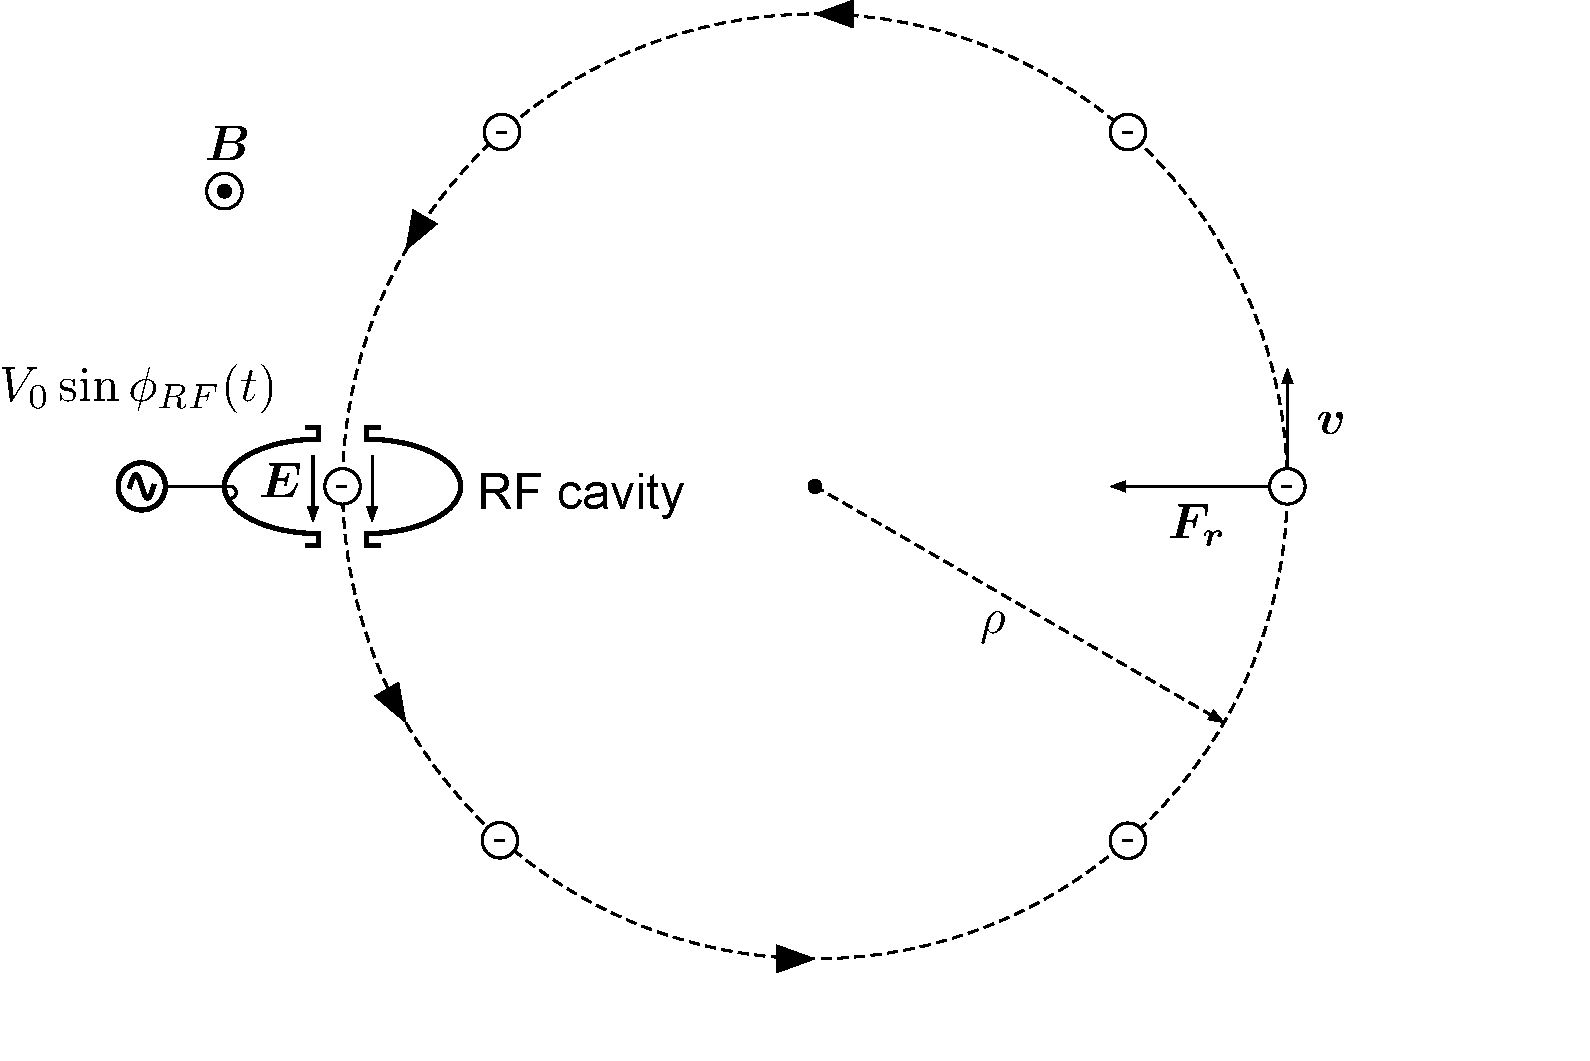
\includegraphics[width=15cm,clip]{rf_circular.pdf}
    \caption{シンクロトロンのモデル}
   \label{rf_circular}
  \end{center}
\end{figure}

粒子の運動方程式は、
%
\begin{equation}
  \frac{d\bm{p}}{dt} = e (\bm{E} + \bm{v}\times \bm{B})
\end{equation}
%
となるが、動径方向の運動を考えると
%
\begin{equation}
  \frac{m v^2}{\rho} = |\bm{F_r}| = e v B
\end{equation}
%
したがって、粒子の運動量と磁場の間には次の関係が成り立つ。
%
\begin{equation}
  p = mv = e \rho B
  \label{momentum}
\end{equation}
%
加速空洞で加速された粒子は運動量が増加するため、同じ軌道を維持するためには (\ref{momentum}) より運動量の変化に応じて磁場$B$を変える必要がある。同様に粒子の速度も増加するため周回周波数$f_0$も高くなるので、それに合わせて加速周波数$f_{RF}$も追随する必要がある。
%
\section{同期粒子}
\begin{figure}[hbt]
  \begin{center}
    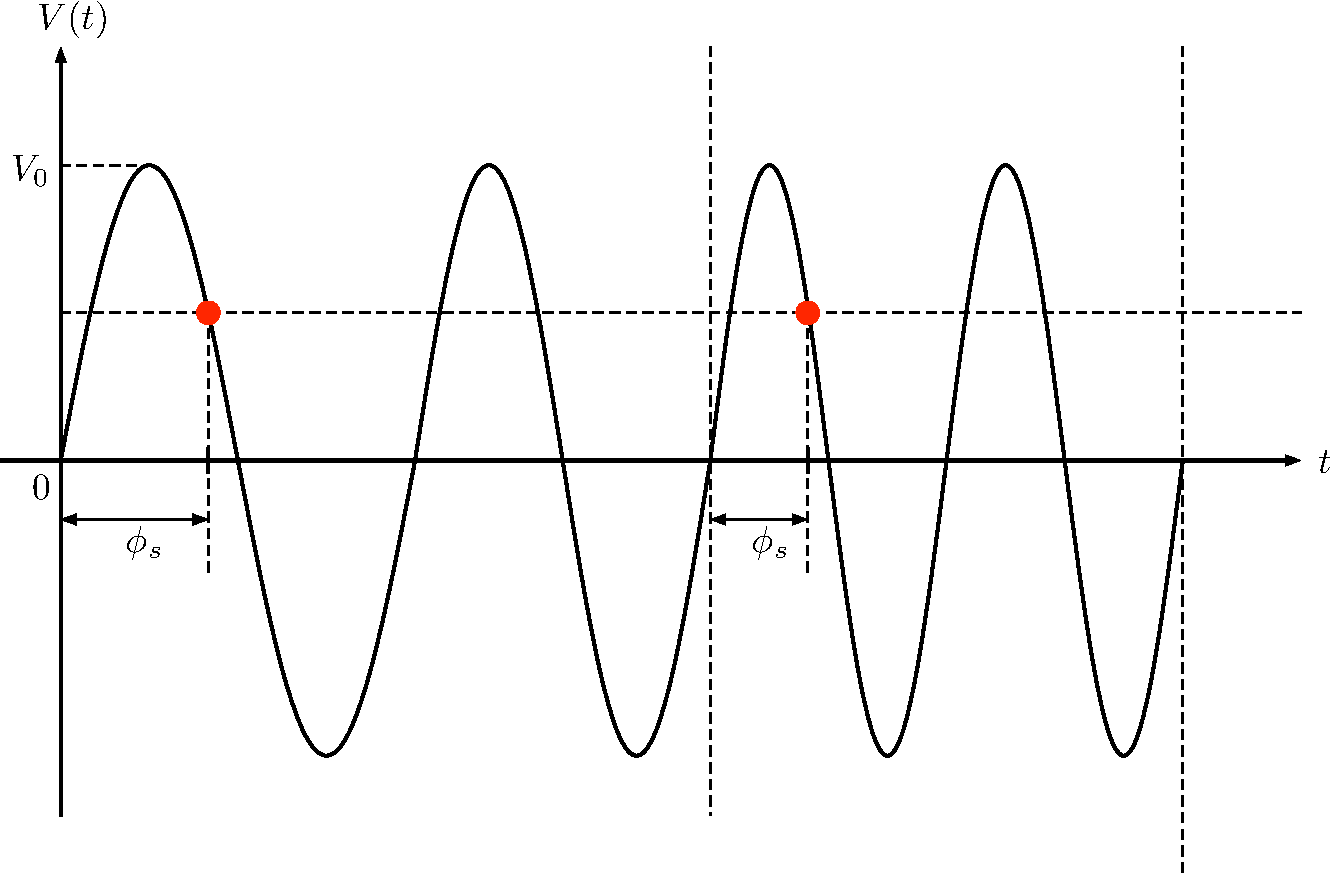
\includegraphics[width=15cm,clip]{synchronous.pdf}
    \caption{$f_{RF} = h f_0$ ($h=2$)}
    \label{synchronous}
  \end{center}
\end{figure}

基準軌道を周回し、毎周同じ位相で加速空洞を通過する粒子を同期粒子 (synchronous particle) と呼び、その位相$\phi_s$のことを同期位相 (synchronous phase) と言う。同期粒子であるためには、周回周波数$f_0$と空洞の加速周波数$f_{RF}$の間に、ある整数$h$を用いて、
%
\begin{equation}
  f_{RF} = h f_0
  \label{harmonic}
\end{equation}
%
という関係が必要である。この整数$h$のことをharmonic numberと言い、加速周波数$f_{RF}$で加速できる最大の粒子数になる。この時、空洞の加速電圧は
%
\begin{equation}
  V_c (t) = V_0 \sin \phi_{RF}(t),\:\phi_{RF}(t) = \int_0^t \omega_{RF}(t) dt
\end{equation}
%
となる。Fig.~\ref{synchronous}は、$h=2$の時の空洞電圧と同期粒子の関係を表してる。

\vspace{\baselineskip}

\begin{tcolorbox}[title=\textgt{SuperKEKBにおける$f_{RF}$, $f_{0}$, $h$}の関係]
  SuperKEKBのリングでは、電子と陽電子は、ほぼ光速$c$で回っており、周長$C_0$は$\SI{3016.315}{\meter}$なので周回周波数$f_0$は
  %
  \begin{equation}
    f_0 = \frac{1}{T_0}=\frac{c}{C_0}=\frac{\SI{2.99792458e8}{\meter / \second}}{\SI{3016.315}{\meter}}=\SI{99.39}{\kilo\hertz} \notag
  \end{equation}
  %
  一方、RF周波数$f_{RF}$は$\SI{508.887}{\mega\hertz}$なので
  %
  \begin{equation}
      f_{RF} = 5120 f_0 \notag
  \end{equation}
  となり、確かに(\ref{harmonic})を満たしている。
\end{tcolorbox}

\section{Dispersion effects in a synchrotron}
粒子の運動量が変化すると、速度や軌道長も変わる。今、運動量偏差 (momentum deviation) を
%
\begin{equation}
  \delta_p = \frac{p-p_0}{p_0}=\frac{\Delta p}{p_0}
\end{equation}
%
とし、同期粒子より運動量が大きい粒子 ($\delta_p >0$) が偏光磁石を通過する場合を考える (Fig.~\ref{dispersion})。
%
\begin{figure}[hbt]
  \begin{center}
    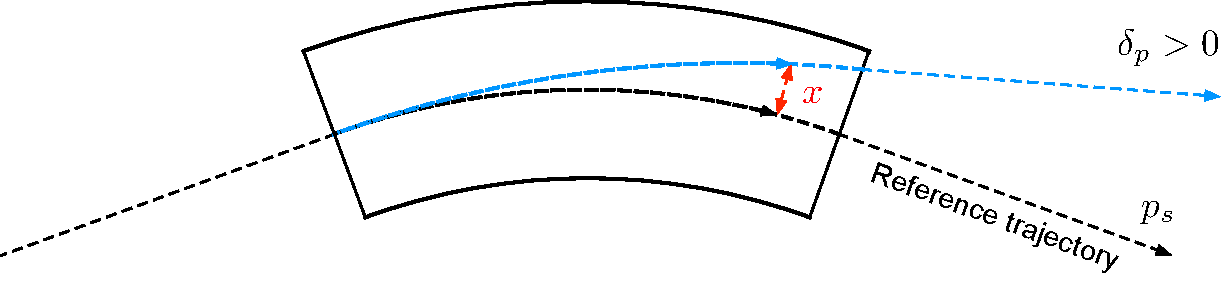
\includegraphics[width=15cm,clip]{dispersion.pdf}
    \caption{Change in path length for a particle in a dipole magnet (with bending radius $\rho$) resulting from the horizontal
    displacement of the particle from the reference trajectory.}
    \label{dispersion}
  \end{center}
\end{figure}
%
その粒子は曲げられにくい為、基準軌道とは異なる軌道を通ることになる。この軌道のずれ$x(s)$は分散関数 (dispersion function) $D_x(s)$を用いて、
%
\begin{equation}
  x(s) = D_x(s)\frac{\Delta p}{p_0} = D_x(s)\delta_p 
\end{equation}
%
と表される。今、基準軌道の曲率半径を$\rho$とすると$ds = \rho d\theta$より、
%
\begin{equation}
  dC = (\rho + x) d\theta = (\rho + x) \frac{ds}{\rho}
\end{equation}
%
したがって、この粒子の軌道長 $C$ は、
%
\begin{align}
  C &= \oint (\rho + x)\frac{ds}{\rho} = \int_0^{C_0} ds + \int_0^{C_0}\frac{x}{\rho} ds \notag \\
  &= C_0 + \delta_p \int_0^{C_0}\frac{D_x(s)}{\rho} ds
\end{align}
%
ここで運動量圧縮率 (momentum compaction factor) $\alpha_p$ を
%
\begin{equation}
  \alpha_p \equiv \frac{1}{C_0} \oint \frac{D_x(s)}{\rho} ds
\end{equation}
%
と定義すると、軌道長の差 $\Delta C = C-C_0$ は、
%
\begin{equation}
  \frac{\Delta C}{C_0}=\alpha_p\frac{\Delta p}{p_0}=\alpha_p\delta_p
  \label{delta_C}
\end{equation}
%
となり$\alpha_p$は運動量の変化による相対的な軌道長の変化を表していることになる。

次に、運動量の変化が回転周期に及ぼす影響を考える事にする。運動量の変化$\Delta p$によって、速度と回転周期がそれぞれ $v=v_0+\Delta v$ と $T=T_0+\Delta T$ に変化した時、回転周期は $T=C/v$ だから、
%
\begin{equation}
  T = T_0 + \Delta T = \frac{C_0 + \Delta C}{v_0 + \Delta v} \notag
\end{equation}
%
分母を払って整理すると、(二次の微小量は無視する)
%
\begin{align}
  & (T_0 + \Delta T)(v_0 + \Delta v) = C_0 + \Delta C \notag \\
  \Longleftrightarrow\quad & \underset{C_0}{\uwave{\cancel{v_0 T_0}}} + \Delta v T_0 + v_0 \Delta T +
  \underset{0}{\uwave{\cancel{\Delta v \Delta T}}}
  = \cancel{C_0} + \Delta C \notag \\
  \Longleftrightarrow\quad & v_0 \Delta T = \Delta C- \Delta v T_0 \notag \\
  \Longleftrightarrow\quad & \frac{\Delta T}{T_0} = \frac{\Delta C_0}{\underset{C_0}{\uwave{v_0 T_0}}} - \frac{\Delta v}{v_0} \notag
\end{align}
%
したがって、
%
\begin{equation}
  \frac{\Delta T}{T_0} = \frac{\Delta C}{C_0} - \frac{\Delta v}{v_0}
  \label{delta_T}
\end{equation}
%
となる。この式より、回転周期の変化 ($\Delta T/T_0$) をもたらす要因として、軌道長の変化 ($\Delta C/C_0$) と粒子の速度の変化 ($\Delta v/v_0$)である事が分かる。ここで(\ref{dv_dp}) より
%
\begin{equation}
  \frac{\Delta v}{v_0}=\frac{1}{\gamma_0^2}\frac{\Delta p}{p_0}
  \label{delta_v}
\end{equation}
%
(\ref{delta_T}) に (\ref{delta_C}) と (\ref{delta_v})を代入すると、
%
\begin{equation}
  \frac{\Delta T}{T_0} = \left(\alpha_p - \frac{1}{\gamma_0^2}\right)\frac{\Delta p}{p_0} = \eta_p \delta_p
  \label{deltat_eta_deltap}
\end{equation}
%
ただし、
%
\begin{equation}
  \eta_p \equiv \alpha_p - \frac{1}{\gamma_0^2} = \frac{1}{\gamma_t^2} - \frac{1}{\gamma_0^2}
  \label{alppha_slip}
\end{equation}
%
はphase slip factorと言い、運動量の変化による相対的な回転周期$T$の変化率を表している。
%

運動量圧縮率が正の場合 ($\alpha_p>0$) を考える。このとき、粒子の運動量を増加させると経路長が増加する。 しかし、粒子の運動量がまだ低く、光度よりも十分遅い場合、粒子の運動量の増加による速度の増加は、運動量の増加による経路長の増加を越えることがあり得る。その結果、粒子の回転周期は短くなる ($\eta_p < 0$)。
一方、粒子の運動量が十分高く超相対論的粒子の場合、粒子の速度は既に光速に十分近く、運動量の増加による速度の増加は極僅かである。この場合、経路長の増加が速度の増加を上回り、粒子の回転周期は長くなる ($\eta_p>0$) 。$\eta_p = 0$の時、つまり
%
\begin{equation}
  \gamma_t = \frac{1}{\sqrt{\alpha_p}}
\end{equation}
%
では回転周期は運動量に依存しない。この$\gamma_t$を遷移エネルギー (transition energy) と言う。

\vspace{\baselineskip}

\begin{tcolorbox}[title=\textgt{SuperKEKB LERのtransition energy}]
  SuperKEKBの陽電子リングLERの運動量圧縮率は$\alpha_p = 3.20 \times 10^{-4}$なので、
  %
  \begin{equation}
    \gamma_t = \frac{1}{\sqrt{\alpha_p}}= \frac{1}{\sqrt{3.20 \times 10^{-4}}} = 55.9 \notag
  \end{equation}
  %
  陽電子の静止質量は$E_0 = \SI{0.5109989461}{\mega\electronvolt}$だから
  \begin{equation}
    E = \gamma_t E_0 = \SI{28.57}{\mega\electronvolt} \notag
  \end{equation}
  %
  となり、入射器からの入射エネルギー$\SI{4}{\giga\electronvolt}$の方がtransition energyより十分高い。
\end{tcolorbox}

\section{位相安定性の原理}
ビームの中には多くの粒子があり、色々な運動量を持つ粒子で構成されている。同期粒子と異なる運動量を持つ粒子が加速空洞を通過する時、どのように加速されるかについて考えてみる。
%
\begin{figure}[hbt]
  \begin{center}
    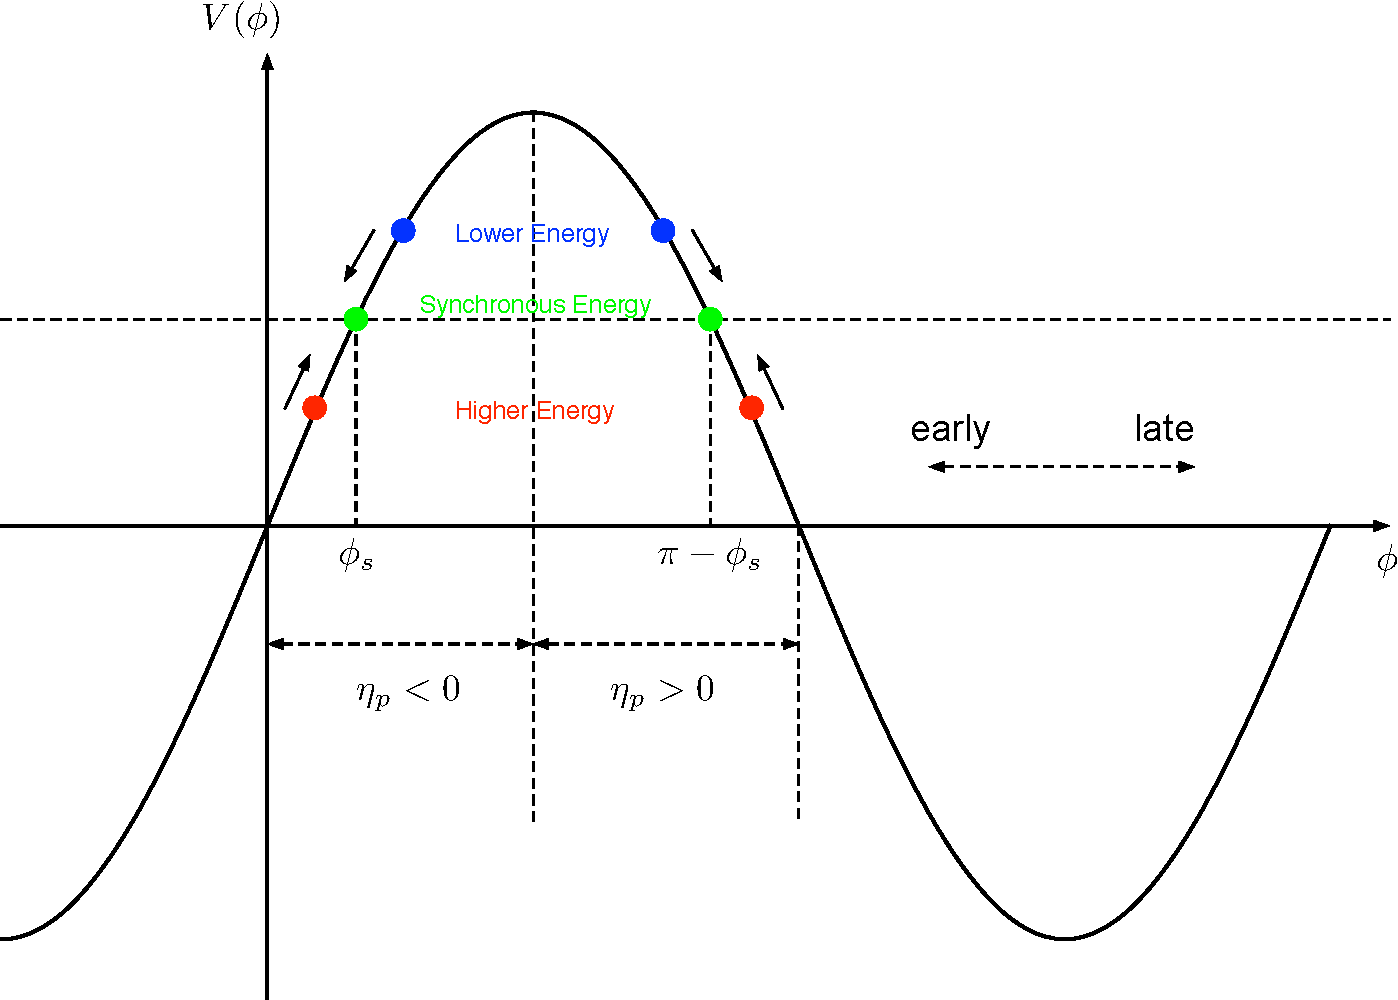
\includegraphics[width=15cm,clip]{phase_stability.pdf}
    \caption{Schematic drawing of an rf wave, and the rf phase angles for a synchronous, a higher, and a lower energy particles.
    For a stable synchrotron motion, the phase focusing principle requires $0 < \phi_s \leq \pi/2$ for $\eta_p < 0$,
    and $\pi/2 < \phi_s \leq \pi$ for $\eta_p > 0$.}
    \label{phase_stability}
  \end{center}
\end{figure}

$\eta_p < 0$ の時、同期粒子より大きい運動量を持つ粒子は、同期粒子より回転周期が短いので、同期粒子より早く加速空洞に到着する。したがって、同期位相$\phi_s$を$0<\phi_s<\pi/2$に選べば、より大きい運動量を持つ粒子は、同期粒子より少ないエネルギーを加速空洞から得ることになる。同様に、同期粒子より小さな運動量を持つ粒子は、同期粒子より遅く加速空洞に到達するので、同期粒子より多いエネルギーを加速空洞から得る。この過程を繰り返すことで、同期粒子の持つ運動量から外れた運動量を持つ粒子は同期粒子の周りを安定に運動することが分かる。$\eta_p > 0$ の時は、同期位相を$\pi/2<\phi_s<\pi$に選べば同様にこの運動は安定である。

\section{Difference Equations for Longitudinal Motion in a Synchrotron}
ここでは、粒子の周回毎の縦方向の運動について考える。リングに加速空洞は一台だけ設置されており、空洞電圧のゼロクロス点からの相対時間を$\tau$、相対位相を$\phi\pmod{2\pi}$とする (Fig.~\ref{coordinates})。今、$n+1$周回目の粒子の空洞への到着時間$\tau(n+1)$と$n$周回目の到着時間$\tau(n)$との差は、粒子の$n+1$周回目の回転周期$T(n+1)$と同期粒子の回転周期$T_0(n+1)$との差に等しいので、
%
\begin{equation}
  \tau(n+1) - \tau(n) = T(n+1) -T_0(n+1)
  \label{tau_T}
\end{equation}
%
\begin{figure}[hhbt]
  \begin{center}
    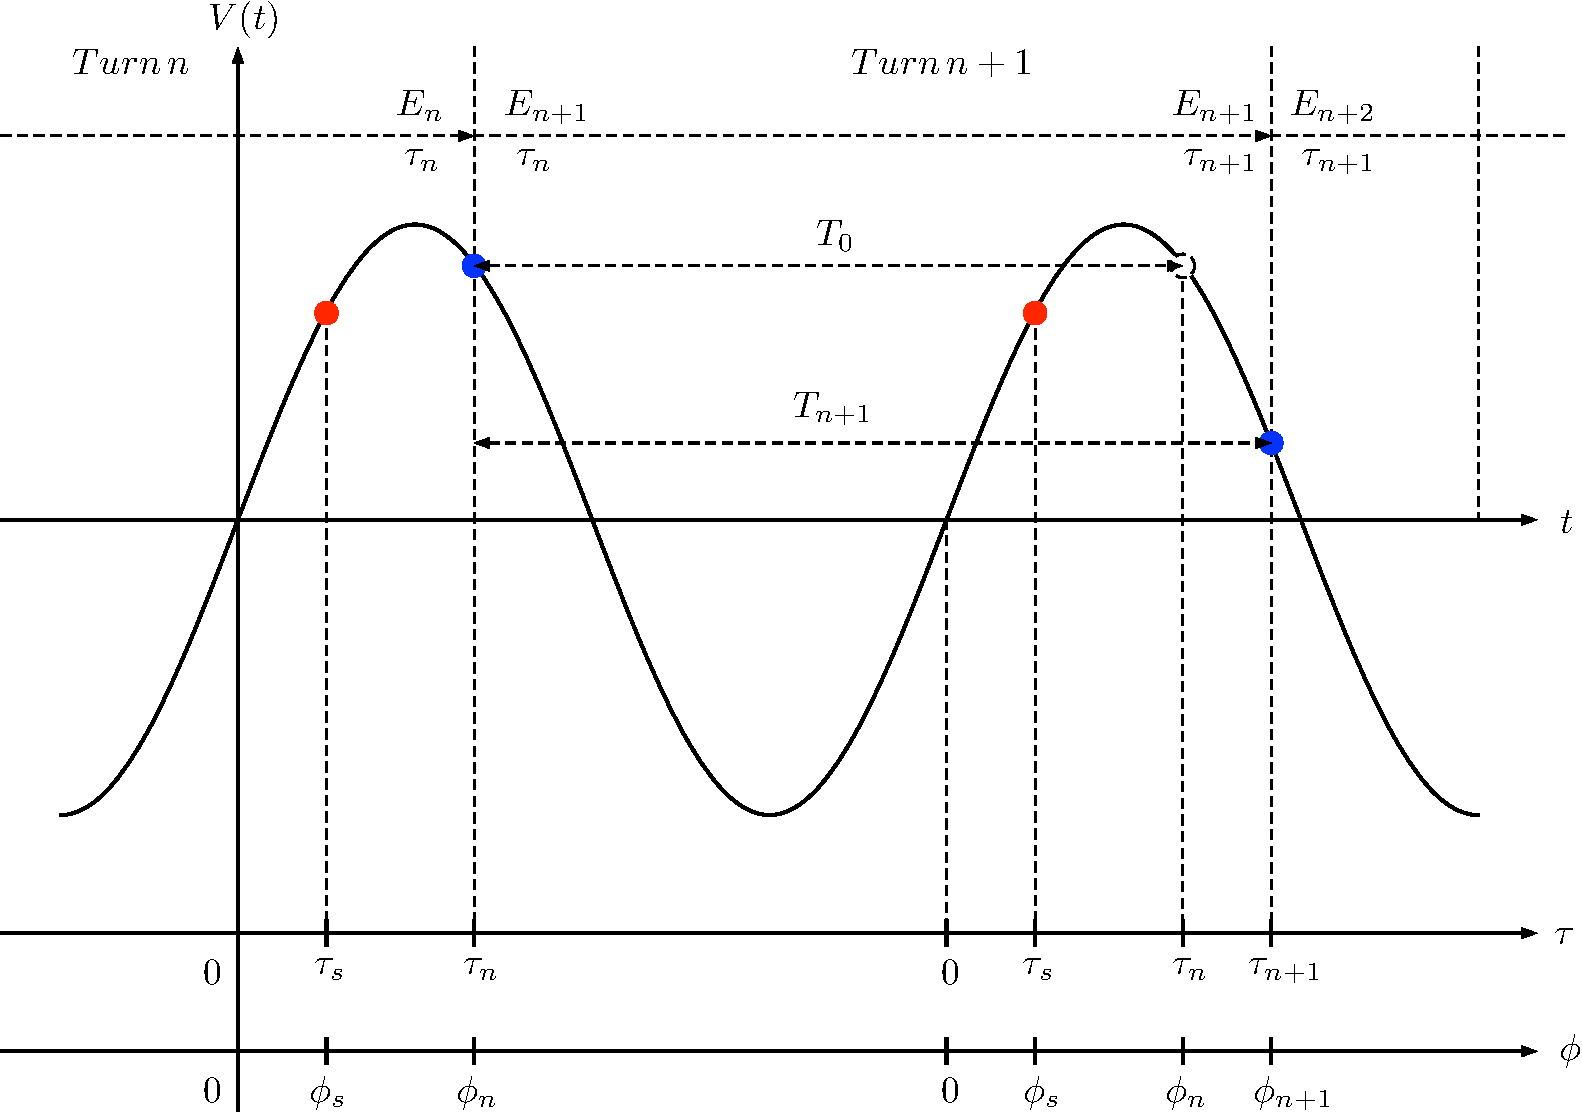
\includegraphics[width=15cm,clip]{coordinates.pdf}
    \caption{Relative and absolute coodinates. ($h=1$)}
    \label{coordinates}
  \end{center}
\end{figure}
%
$\phi(n+1) = \omega_{RF}(n+1) \tau(n+1)$から、この関係を用いると、
%
\begin{align}
  \phi(n+1) &=\omega_{RF}(n+1)\{\tau(n) + T(n+1) -T_0(n+1)\} \notag \\
    &= \frac{\omega_{RF}(n+1)}{\omega_{RF}(n)} \phi(n) + \omega_{RF}(n+1)\{T(n+1) -T_0(n+1)\}  \notag
\end{align}
%
ここで、(\ref{deltat_eta_deltap})より、
%
\begin{equation}
    \frac{T(n+1)-T_0(n+1)}{T_0(n+1)} = \eta \delta_p(n+1)
\end{equation}
%
を用いると、
%
\begin{align}
  \phi(n+1) &= \frac{\omega_{RF}(n+1)}{\omega_{RF}(n)}\phi(n) + \omega_{RF}(n+1)T_0(n+1)\eta \delta_p(n+1) \notag \\
  &=\frac{\omega_{RF}(n+1)}{\omega_{RF}(n)}\phi(n) + 2\pi h \eta \delta_p(n+1)
\end{align}
%
ここで、
%
\begin{equation}
  \frac{\omega_{RF}(n+1)}{\omega_{RF}(n)} \approx 1
\end{equation}
%
という近似を行うと、
%
\begin{equation}
  \phi(n+1) = \phi(n) + 2\pi h \eta \delta_p(n+1)
\end{equation}

次に、$n+1$周回目の粒子のエネルギー$E(n+1)$は、$E(n)$に位相$\phi(n)$で空洞を通過する時に得られるエネルギーを足し合わせたものだから、
%
\begin{equation}
  E(n+1) = E(n) + e V \sin\phi (n)
\end{equation}
%
同期粒子に関しても同様に考えると、
%
\begin{equation}
  E_0(n+1) = E_0(n) + e V \sin\phi_s
\end{equation}
%
両辺の差を取り、$\Delta E = E - E_0$とすると、
%
\begin{equation}
  \Delta E(n+1) = \Delta E(n) + e V (\sin\phi(n) - \sin\phi_s)
\end{equation}
%
ここで、(\ref{dp_de})より、
%
\begin{equation}
  \delta_p = \frac{\Delta p}{p_0} = \frac{1}{\beta_0^2}\frac{\Delta E}{E_0}
  \label{delta_p}
\end{equation}
%
より、
%
\begin{equation}
  \Delta E(n+1) - \Delta E(n) = \beta^2 E_0 \{\delta_p(n+1) - \delta_p(n)\}
\end{equation}
%
したがって、
%
\begin{equation}
  \delta_p(n+1) - \delta_p(n) = \frac{e V}{\beta_0^2 E_0}(\sin\phi(n) -\sin\phi_s)
\end{equation}
%

以上より、シンクロトロンの縦方向の運動について、周回毎の差分方程式
%
\begin{align}
  \begin{split}
     &\delta_p(n+1) = \delta_p(n) + \frac{e V}{\beta_0^2 E_0}(\sin\phi(n) -\sin\phi_s) \\
     &\phi(n+1) = \phi(n) + 2\pi h \eta \delta_p(n+1)
    \label{map}
  \end{split}
\end{align}
%
が導かれた。これらの式を使ってparticle tracking simulationを行うことができる。

\section{Differential Equations for Longitudinal Motion in a Synchrotron}
The difference equations (\ref{map}) can be written as continuous differential equations, if the assumption is made that the change of the variables $\phi$ and $\delta_p$ during one turn in the ring is not too large. In this case, the difference quotient can be approximated by the differential quotient
%
\begin{equation}
    \frac{\delta_p(n+1)-\delta_p(n)}{T_0(n+1)} \approx \frac{d\delta_p}{dt}=\dot{\delta_p},\quad 
    \frac{\phi(n+1)-\phi(n)}{T_0(n+1)} \approx \frac{d\phi}{dt}= \dot{\phi}
\end{equation}
%
\begin{align}
    \begin{split}
        \dot{\delta_p} &= \frac{e V \omega_0}{2\pi \beta_0^2 E_0}(\sin\phi - \sin\phi_s) \\
        \dot{\phi} &= h \omega_0 \eta \delta_p
    \end{split}
\end{align}
%
\begin{equation}
    \ddot{\phi} = \frac{e V h \eta \omega_0^2}{2\pi\beta_0^2 E_0}(\sin\phi-\sin\phi_s)
\end{equation}
%
\subsection{Small amplitude approximation}
$\Delta\phi = \phi - \phi_s$が非常に小さい時、
%
\begin{equation}
    \sin\phi = \sin(\phi_s+\Delta\phi) \approx \sin\phi_s + \cos\phi_s \Delta\phi
\end{equation}
%
より
%
\begin{equation}
    \ddot{\Delta\phi} = \frac{e V h \eta \omega_0^2}{2\pi \beta_0^2 E_0} \cos\phi_s \Delta\phi = - \omega_s^2 \Delta\phi
\end{equation}
%
ただし、
%
\begin{equation}
    \omega_s = \sqrt{-\frac{e V h \eta \omega_0^2 \cos\phi_s}{2\pi \beta_0^2 E_0}}
\end{equation}
%
\clearpage

\appendix
\renewcommand{\theequation}{\Alph{section}.\arabic{equation} }
\setcounter{equation}{0}

\section{相対論のおさらい}
\begin{equation}
    E_0 = m_0 c^2 ,\quad E = \sqrt{E_0^2 + p^2 c^2}
\end{equation}

\begin{equation}
    \beta = \frac{v}{c}\,,\quad \gamma = \frac{E}{E_0}=\frac{m}{m_0}=\frac{1}{\sqrt{1-\beta^2}}
\end{equation}

\begin{equation}
    p = mv = \gamma m_0 v = \gamma m_0 \beta c
\end{equation}

\begin{equation}
    \frac{p}{E} = \frac{\gamma m_0 \beta c}{\gamma m_0 c^2} = \frac{\beta}{c}
\end{equation}

\paragraph{(\ref{delta_v}) の導出}

\begin{equation}
  \frac{dp}{dv} = m_0\frac{d}{dv}(\gamma v)
  = m_0 \left(\gamma + v \frac{d\gamma}{dv}\right) \notag
\end{equation}
%
\begin{align}
  \frac{d\gamma}{dv} & = \frac{1}{c}\frac{d\gamma}{d\beta}= \frac{1}{c}\frac{d}{d\beta}\left(\frac{1}{\sqrt{1-\beta^2}}\right) \notag \\
  & = \frac{1}{c} \beta \underset{\gamma^{-2}}{\uwave{(1-\beta^2)}}^{-\frac{3}{2}} = \frac{\beta \gamma^3}{c} \notag
\end{align}
%
これより、
\begin{align}
  \frac{dp}{dv} & = m_0 \left(\gamma + v \frac{\beta \gamma^3}{c}\right)
  = m_0 \gamma \underset{\gamma^2}{\uwave{(1 + \beta^2 \gamma^2)}}
  = \frac{\gamma^2 p}{v} \notag
\end{align}
%
したがって、
%
\begin{equation}
  \quad \frac{dv}{v} = \frac{1}{\gamma^2}\frac{dp}{p}
  \label{dv_dp}
\end{equation}
%
\paragraph{(\ref{delta_p})の導出}
%
\begin{align}
  p = mv = \gamma m_0 \beta c\,  , \quad E = \gamma E_0 = \gamma m_0 c^2 \notag
\end{align}
%
\begin{equation}
  \gamma \beta = \gamma \sqrt{1-\frac{1}{\gamma^2}} \notag = \sqrt{\gamma^2 -1} \notag
\end{equation}
%
\begin{align}
  \frac{dp}{dE} & = \frac{1}{c}\frac{d(\gamma \beta)}{d\gamma} = \frac{1}{c}\frac{d}{d\gamma}\sqrt{\gamma^2 -1} \notag \\
  & = \frac{\gamma}{c} \underset{\gamma^2\beta^2}{(\uwave{\gamma^2 -1}})^{-\frac{1}{2}} = \frac{1}{c\beta}
  = \frac{p}{\beta^2 E}\notag
\end{align}
%
したがって、
%
\begin{equation}
  \quad \frac{dp}{p} = \frac{1}{\beta^2}\frac{dE}{E}
  \label{dp_de}
\end{equation}

%
\begin{thebibliography}{9}
  \bibitem{Chao}
  A. Chao, K. Mess, M. Tigner, and F. Zimmermann, Handbook of Accelerator Physics and Engineering (2nd Edition), World Scientific Publishing Company Incorporated, Singapore (2013)
  \bibitem{a}
  A.W.Chao and M.Tigner,editors.Handbook of Accelerator Physics and Engineering. World Scientific Pub. Co., 3rd printing edition, 2009.
  \bibitem{Wolski}
  Andy Wolski, Beam Dynamics in High Energy Particle Accelerators,  Imperial College Pr (2014).
  \bibitem{Lee}
  S. Y. Lee, Accelerator physics, World Scientific (2004), ISBN 9789812562005.
  \bibitem{Edwards}
  D.A. Edwards, M.J. Syphers, `An introduction to the physics of high energy accelerators', Wiley (1993).
\end{thebibliography}
%
\end{document}